\documentclass[a4paper,11pt,oneside,openany]{book}
\usepackage{styles/handbook}
\hypersetup{pdftitle={第一批验收样章：神经网络基础}}
\begin{document}
\frontmatter
\hypersetup{pageanchor=false}
\begin{titlepage}
\vspace*{16mm}
{\sffamily\color{Teal}\large 机器学习与深度学习：图解速查手册\par}
\vspace{15mm}
{\sffamily\bfseries\color{Ink}\Huge 神经网络基础\par}
\vspace{6mm}
{\sffamily\color{Ink}\LARGE 从结构到一次参数更新\par}
\vspace{12mm}
\noindent\textcolor{Teal}{\rule{\textwidth}{1.2pt}}
\vspace{7mm}
\begin{keyidea}[第一批验收样章]
本批逐张核查了 12 张原始速查图，将其知识主题合并成连贯章节。
图表重新绘制，补充了符号、条件、读图说明和可复算的例子。
本文件仅包含这一批样章；完整工作稿仍在修订中。
\end{keyidea}
\vfill
原项目作者：张海飞、郭金珊、任露芹、李慧、朱靖、朱弘毅\par
\vspace{4mm}
2026年10月28日\par
\end{titlepage}
\hypersetup{pageanchor=true}
\tableofcontents
\mainmatter
\chapter{神经网络：从结构到一次参数更新}
\label{ch:neural}
\noindent{\sffamily\small\color{Teal}第二部分 · 深度学习基础}\par\smallskip

神经网络（Neural Network）把一系列可调的数学变换组合起来，将输入映射为预测。
学习的关键，是利用数据调整这些变换中的参数，而不是手工规定每个中间特征。
本章围绕一个问题展开：\textbf{一次预测出错后，网络怎样知道该调整哪些参数？}

\begin{keyidea}[本章阅读路线]
先看网络如何计算预测，再选择输出与损失，最后把损失的梯度传回各层并更新参数。
需要的数学只有加权求和、矩阵乘法、导数和链式法则。
本章用列向量表示单个样本；$n$ 表示样本数，$d$ 表示输入特征数，$K$ 表示类别数。
\end{keyidea}

\section{把训练过程连起来}
\label{sec:training-map}

训练一个监督学习网络，需要训练数据、网络结构、损失函数和优化方法。
损失函数回答“当前预测错了多少”，反向传播回答“参数改变会怎样影响损失”，
优化器根据梯度决定“这一步怎样改参数”。

\begin{figure}[htbp]
\centering
\begin{tikzpicture}[node distance=6mm and 7mm]
\node[box,text width=29mm] (data) {训练集\\$\{(\vct x_i,y_i)\}$};
\node[box,text width=29mm,right=of data] (model) {网络 $f_\theta$\\前向计算};
\node[box,text width=29mm,right=of model] (loss) {损失 $J(\theta)$\\衡量预测偏差};
\node[box,text width=29mm,below=of loss] (grad) {反向传播\\计算梯度};
\node[box,text width=29mm,left=of grad] (update) {优化器\\更新参数 $\theta$};
\draw[flow] (data)--(model);
\draw[flow] (model)--(loss);
\draw[flow] (loss)--(grad);
\draw[flow] (grad)--(update);
\draw[flow] (update)--(model);
\node[box,text width=29mm,left=of update,draw=Amber,fill=Amber!5] (val) {验证集\\选择训练方案};
\draw[flow,draw=Amber,dashed] (model.south west)--(val.north east);
\end{tikzpicture}

\caption{训练循环与验证的分工。虚线表示用验证数据评估方案，不通过该分支拟合参数。}
\label{fig:training-map}
\par\smallskip
\readfigure{沿实线走一圈，就是一次参数更新。网络先产生预测，损失把预测与标签比较，
反向传播计算梯度，优化器据此更新参数，随后才能开始下一次计算。
验证集用来选择网络宽度、学习率或停止时刻；测试集留到方案确定后评估。}
\end{figure}

对于训练集 $\mathcal D=\{(\vct x_i,y_i)\}_{i=1}^n$，一个常见目标是
\begin{equation}
 J(\theta)=\frac1n\sum_{i=1}^n\ell\bigl(f_\theta(\vct x_i),y_i\bigr)
              +\lambda\Omega(\theta).
 \label{eq:nn-objective}
\end{equation}
这里 $\theta$ 是网络全部可训练参数，$f_\theta$ 是预测模型，$\ell$ 是单个样本的损失，
$\Omega$ 是正则化项，$\lambda\geq0$ 控制正则化强度。
本章手算例子令 $\lambda=0$，便于看清计算过程。

\begin{pitfall}
测试集不参与参数拟合、阈值选择或学习率调整。
归一化、缺失值填补等需要从数据估计的步骤，也只能先在训练数据上拟合，
再应用于验证集和测试集。训练损失下降，并不保证新数据上的误差下降。
\end{pitfall}

\section{结构、前馈与隐藏层}
\label{sec:nn-structure}

前馈神经网络（Feedforward Neural Network）的计算连接不形成有向环。
全连接的多层感知机（Multilayer Perceptron, MLP）是其中一种常见形式：
相邻层的每个单元与上一层的全部单元相连。
卷积网络也可以是前馈网络，所以“前馈网络”和“MLP”不能在所有语境下画等号。

\begin{figure}[htbp]
\centering
\begin{tikzpicture}[x=30mm,y=11mm]
\foreach \i in {1,2,3}{\node[unit] (i\i) at (0,\i) {$x_{\i}$};}
\foreach \i in {1,2,3,4}{\node[unit] (h\i) at (1.5,\i-0.5) {};}
\foreach \i in {1,2,3}{\node[unit] (g\i) at (3,\i) {};}
\node[unit,fill=Teal!20] (o) at (4.5,2) {$\hat y$};
\begin{scope}[on background layer]
\foreach \i in {1,2,3}{\foreach \j in {1,2,3,4}{\draw[flow,thin,Teal!40] (i\i)--(h\j);}}
\foreach \i in {1,2,3,4}{\foreach \j in {1,2,3}{\draw[flow,thin,Teal!40] (h\i)--(g\j);}}
\foreach \i in {1,2,3}{\draw[flow,thin,Teal!40] (g\i)--(o);}
\end{scope}
\node[lab] at (0,-0.4) {输入层：3};
\node[lab] at (1.5,-0.4) {隐藏层：4};
\node[lab] at (3,-0.4) {隐藏层：3};
\node[lab] at (4.5,-0.4) {输出层：1};
\draw[flow] (0,4.4)--node[above,lab]{前向计算：输入到输出}(4.5,4.4);
\end{tikzpicture}

\caption{一个 $3\!\to\!4\!\to\!3\!\to\!1$ 的 MLP。箭头表示计算依赖，偏置未画出。}
\label{fig:network}
\par\smallskip
\readfigure{最左侧的三个输入单元只是三个特征的入口。
中间两列分别有四个和三个隐藏单元，最右侧只有一个输出。
每条连接对应一个权重；每个隐藏单元和输出单元通常还有一个偏置。
这些偏置不应因为图中省略而在计算时被忘掉。}
\end{figure}

\textbf{隐藏层（Hidden Layer）}位于输入与输出之间，其激活值是网络根据输入计算出的中间表示。
“隐藏”指它们没有直接作为任务所给定的输入或目标，并不表示它们无法观察，也不表示必须另有标签。
它们会在后续训练中通过最终损失的梯度间接得到调整。

\textbf{宽度（Width）}描述一层有多少单元；\textbf{深度（Depth）}描述计算经过多少层。
本书计算参数层数时不计输入层，因此图中的网络有三个参数层、两个隐藏层。
其他资料可能采用不同的计数约定，比较结构时应先确认口径。

这个网络的可训练参数总数为
\[
 (3\times4+4)+(4\times3+3)+(3\times1+1)=35.
\]
每个括号中的前一项数连接权重，后一项数偏置。
输入层没有要在这里拟合的权重或偏置。

\begin{keyidea}[结构由什么决定？]
输入维度由数据表示决定，输出形式由任务决定；隐藏层的层数、宽度和激活函数是建模选择。
可以在验证集上比较候选结构，但不存在对所有数据都最优的网络深度。
更多层或更多参数带来表达能力与计算成本的变化，不自动带来更好的泛化。
\end{keyidea}

\section{神经元与前向计算}
\label{sec:nn-forward}

人工神经元（Artificial Neuron）可以看成“加权求和，加偏置，再做激活”的小计算模块。
权重决定输入各分量怎样组合，偏置决定变换的平移，激活函数改变组合结果的形状。

\begin{figure}[htbp]
\centering
\begin{tikzpicture}[node distance=7mm and 8mm]
\node[box,text width=24mm] (x) {输入\\$x_1,\ldots,x_d$};
\node[box,text width=42mm,right=of x] (sum) {加权求和并加偏置\\$z=\sum_j w_jx_j+b$};
\node[box,text width=25mm,right=of sum] (act) {激活\\$a=\phi(z)$};
\node[right=of act,lab] (out) {输出 $a$};
\draw[flow] (x)--(sum);
\draw[flow] (sum)--(act);
\draw[flow] (act)--(out);
\end{tikzpicture}

\caption{单个神经元的计算。偏置在激活之前加入。}
\label{fig:neuron}
\par\smallskip
\readfigure{输入先乘各自权重并相加，得到激活前的数值 $z$；
激活函数 $\phi$ 将 $z$ 转为输出 $a$。图中的“求和”并非把输入原样相加，而是进行加权求和。}
\end{figure}

\subsection{先算一个单元}
设 $\vct x=(2,-1)^\top$、$\vct w=(0.5,1)^\top$、$b=0.2$，则
\[
 z=\vct w^\top\vct x+b=0.5\times2+1\times(-1)+0.2=0.2.
\]
若用 ReLU，输出为 $a=0.2$；若用 Sigmoid，输出约为 $a=0.550$。
相同的加权输入，经过不同的激活函数会产生不同的输出。

\subsection{一层就是多个单元一起算}
记第 $l$ 层有 $d_l$ 个单元，$\vct a^{(0)}=\vct x$。前向传播写为
\begin{equation}
 \vct z^{(l)}=W^{(l)}\vct a^{(l-1)}+\vct b^{(l)},\qquad
 \vct a^{(l)}=\phi^{(l)}\bigl(\vct z^{(l)}\bigr).
 \label{eq:nn-forward}
\end{equation}
对逐元素激活，每个单元只对自己的 $z$ 做变换。Softmax 是向量变换，需把整组输出一起计算。

\begin{center}
\small
\begin{tabularx}{0.96\textwidth}{l l X}
\toprule
对象 & 形状 & 含义\\
\midrule
$\vct a^{(l-1)}$ & $d_{l-1}\times1$ & 上一层输出\\
$W^{(l)}$ & $d_l\times d_{l-1}$ & 每一行对应当前层一个单元的权重\\
$\vct b^{(l)}$ & $d_l\times1$ & 当前层偏置\\
$\vct z^{(l)},\vct a^{(l)}$ & $d_l\times1$ & 当前层激活前的值与激活值\\
\bottomrule
\end{tabularx}
\end{center}

\quick{先检查矩阵形状，再计算数值。隐藏层在计算新的表示；输出层把表示转换成任务所需的预测。}

\section{为什么需要非线性激活？}
\label{sec:nn-activations}

如果每层都只有仿射变换，堆叠后仍然只是仿射变换。例如
\[
 W_2(W_1\vct x+\vct b_1)+\vct b_2
   =(W_2W_1)\vct x+(W_2\vct b_1+\vct b_2).
\]
因此，仅增加这样的层数无法获得一般的非线性表达能力。
激活函数（Activation Function）让网络能表示更丰富的关系。

\begin{figure}[htbp]
\centering
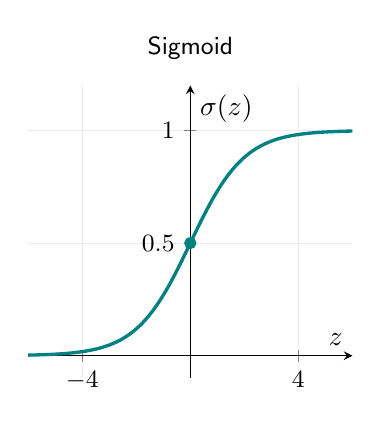
\begin{tikzpicture}
\begin{axis}[width=0.47\textwidth,height=53mm,axis lines=middle,
  xmin=-6,xmax=6,ymin=-0.1,ymax=1.2,xlabel={$z$},ylabel={$\sigma(z)$},
  xtick={-4,0,4},ytick={0.5,1},tick label style={font=\small},
  title={Sigmoid},title style={font=\small\sffamily},grid=major,grid style={gray!15}]
\addplot[Teal,very thick,domain=-6:6,samples=100]{1/(1+exp(-x))};
\addplot[only marks,mark=*,Teal] coordinates {(0,0.5)};
\end{axis}
\end{tikzpicture}\hfill
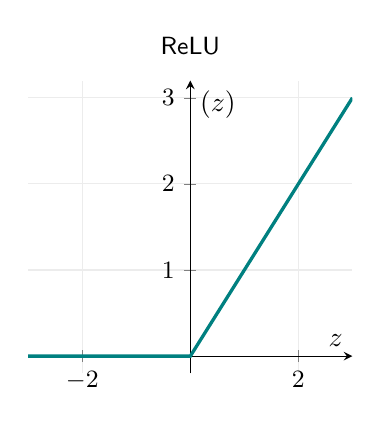
\begin{tikzpicture}
\begin{axis}[width=0.47\textwidth,height=53mm,axis lines=middle,
  xmin=-3,xmax=3,ymin=-0.2,ymax=3.2,xlabel={$z$},ylabel={$\ReLU(z)$},
  xtick={-2,0,2},ytick={1,2,3},tick label style={font=\small},
  title={ReLU},title style={font=\small\sffamily},grid=major,grid style={gray!15}]
\addplot[Teal,very thick] coordinates {(-3,0)(0,0)(3,3)};
\end{axis}
\end{tikzpicture}

\caption{Sigmoid 平滑地压缩数值；ReLU 保留正半轴，把负半轴置零。}
\label{fig:activations}
\par\smallskip
\readfigure{左图过 $(0,0.5)$ 且单调递增，两端逐渐变平；
右图在原点折转，负半轴为水平线，正半轴斜率为 1。
曲线的斜率就是反向传播会用到的局部导数。}
\end{figure}

\begin{align}
 \sigma(z)&=\frac{1}{1+e^{-z}}, & \sigma'(z)&=\sigma(z)(1-\sigma(z)),\label{eq:sigmoid}\\
 \ReLU(z)&=\max(0,z), & \ReLU'(z)&=
 \begin{cases}0,&z<0,\\1,&z>0.\end{cases}\label{eq:relu}
\end{align}

\textbf{Sigmoid：}有限实数输入的输出严格位于 $(0,1)$，适合表示单个二元事件的概率估计。
其导数不超过 $1/4$；当 $|z|$ 很大时导数趋近于 0，但在有限实数处不等于 0。
多层连乘小导数可能使梯度变小，因而 Sigmoid 通常不是深层隐藏层的默认选择。

\textbf{修正线性单元（Rectified Linear Unit, ReLU）：}计算简单，正半轴的导数为 1，
是隐藏层常见的起点。$z=0$ 处经典导数不存在，实际自动求导通常约定取 0。
如果一个单元对训练输入长期都输出 0，其输入侧参数可能难以再更新，这称为“死亡 ReLU”。

\begin{pitfall}
ReLU 不能保证整个深层网络不会出现梯度消失。
梯度还受到权重、网络深度、输入分布等因素影响。
Sigmoid 输出的数值也不会仅因位于 $(0,1)$ 就自动成为校准良好的概率。
\end{pitfall}

\section{XOR：隐藏表示怎样改变可分性}
\label{sec:nn-xor}
异或（XOR）在两个输入不同的时候输出1，相同时输出0。
四个输入$(0,0),(1,0),(0,1),(1,1)$的目标为$0,1,1,0$；
它们不能由原平面中的一条直线严格分开。

\begin{figure}[H]
\centering\begin{tikzpicture}
\begin{axis}[width=68mm,height=58mm,xmin=-.3,xmax=1.3,ymin=-.3,ymax=1.3,
 xlabel={$x_1$},ylabel={$x_2$},xtick={0,1},ytick={0,1},title={原输入：一条直线无法分开}]
\addplot[only marks,mark=*,Teal,mark size=3pt] coordinates {(1,0)(0,1)};
\addplot[only marks,mark=square*,Amber,mark size=3pt] coordinates {(0,0)(1,1)};
\end{axis}
\begin{axis}[at={(79mm,0)},anchor=south west,width=68mm,height=58mm,xmin=-.3,xmax=1.3,ymin=-.3,ymax=1.3,
 xlabel={$h_1=\ReLU(x_1-x_2)$},ylabel={$h_2=\ReLU(x_2-x_1)$},xtick={0,1},ytick={0,1},title={新表示：按$h_1+h_2$分开}]
\addplot[Quiet,dashed,domain=-.2:.7]{.5-x};
\addplot[only marks,mark=*,Teal,mark size=3pt] coordinates {(1,0)(0,1)};
\addplot[only marks,mark=square*,Amber,mark size=3pt] coordinates {(0,0)};
\end{axis}
\end{tikzpicture}

\caption{青色圆点为正类，橙色方点为负类；两负类在隐藏表示中重合到原点。}
\end{figure}
\readfigure{设$h_1=\ReLU(x_1-x_2)$、$h_2=\ReLU(x_2-x_1)$，
则正类映为$(1,0)$或$(0,1)$，负类均为$(0,0)$。
再按$h_1+h_2>0.5$即可分类。这里显式构造权重，说明表示能力，不等于保证训练自动找到它。}

若所有层都只有仿射变换，$W_2(W_1x+b_1)+b_2$
仍是一个仿射变换；单纯叠层没有引入这里所需的非线性表达。
中间的非线性使组合获得不同形状的决策边界。

深度可让某些具有组合结构的函数更高效地表示，并不意味着越深越好。
常见通用逼近结论有函数、区域与网络宽度等条件，也不保证优化、样本需求或测试泛化。
XOR只需很小的隐藏表示，不需要很深的网络。

\quick{先问结构能否表达，再问优化能否学到，最后问新数据是否有效；三个问题不能相互替代。}


\section{Softmax：把一组得分变为分布}
\label{sec:nn-softmax}

当一个样本必须属于 $K$ 个互斥类别中的某一个时，
网络通常先输出 $K$ 个实数得分，称为 logits。
Softmax 将这组得分转换为和为 1 的概率分布估计：
\begin{equation}
 p_k=\softmax(\vct z)_k=\frac{e^{z_k}}{\sum_{j=1}^K e^{z_j}},
 \qquad k=1,\ldots,K.
 \label{eq:softmax}
\end{equation}
对有限 logits，所有 $p_k>0$ 且 $\sum_k p_k=1$。
分母遍历同一个样本的全部类别，而不是遍历不同样本。

\begin{figure}[htbp]
\centering
\begin{tikzpicture}[node distance=6mm and 9mm]
\node[box,text width=32mm] (z) {原始得分（logits）\\$\vct z=(2,1,0)$};
\node[box,text width=38mm,right=of z] (shift) {减去最大值后取指数\\$(1,e^{-1},e^{-2})$};
\node[box,text width=39mm,right=of shift] (p) {除以总和\\$(0.665,0.245,0.090)$};
\draw[flow] (z)--(shift);
\draw[flow] (shift)--(p);
\end{tikzpicture}

\caption{三分类的数值例子。显示值经过四舍五入。}
\label{fig:softmax}
\par\smallskip
\readfigure{得分最大的第一类获得最高概率，但其概率约为 $0.665$，并不接近 1。
第二、三类仍保有概率质量。若取概率最大的类别作为最终标签，这一步才是离散的分类决策。}
\end{figure}

\subsection{数值稳定性来自平移不变性}
若给每个得分同时减去常数 $c$，分子分母会约去相同的因子 $e^{-c}$，所以结果不变。
通常取 $c=\max_j z_j$：
\begin{equation}
 p_k=\frac{e^{z_k-c}}{\sum_j e^{z_j-c}}.
 \label{eq:stable-softmax}
\end{equation}
这样所有指数的输入都不大于 0，避免直接计算过大的指数。
图中的 $(2,1,0)$ 与 $(1002,1001,1000)$ 应当得到相同的分布。
极小分量仍可能在有限精度下下溢；需要对数概率时，应直接使用稳定的 log-softmax 计算。

\begin{keyidea}[Softmax 会不会总选出一个接近 1 的概率？]
不会。若所有得分相等，每类概率都是 $1/K$；差距越大，分布才可能越集中。
Softmax 保持得分的大小顺序，\textbf{它不是取最大值运算，也不是概率校准的保证}。
例如把 $\vct z$ 乘以一个较大的正数，会改变概率集中程度，却不改变最高分的类别。
\end{keyidea}

\quick{Sigmoid 逐个处理二元事件；Softmax 联合处理互斥类别。判断任务能否同时有多个真标签，再选择输出。}

\section{把输出层和损失函数配对}
\label{sec:nn-output}

输出层的形式由预测目标决定，不能只根据“分类”两个字选择。
例如，一张图片的主类别若必须从猫、狗、鸟中选一个，是互斥多分类；
若同时判断“有动物”“在室外”“有车辆”，则是多标签分类（Multilabel Classification）。

\begin{center}
\small
\renewcommand{\arraystretch}{1.35}
\begin{tabularx}{\textwidth}{P{30mm}P{22mm}Y P{29mm}}
\toprule
任务 & 输出维度 & 预测时常见变换 & 常见损失\\
\midrule
无约束实值回归 & 目标数 & 恒等映射（线性输出） & 均方误差\\
二分类 & 1 & Sigmoid & 二元交叉熵\\
互斥多分类 & $K$ & Softmax & 类别交叉熵\\
多标签分类 & 标签数 $K$ & 每个分量分别用 Sigmoid & 逐标签二元交叉熵\\
\bottomrule
\end{tabularx}
\end{center}

\textbf{读表：}维度是每个样本输出的数值个数。
多标签任务的概率不必加起来等于 1；无约束实值回归才通常采用线性输出。
正值目标、计数或其他带约束的目标，需要结合其统计模型选择输出和损失。
二分类也能采用两个 logits 的 Softmax，这里列出的是更紧凑的一输出形式。

\subsection{二元交叉熵（Binary Cross-Entropy, BCE）}
对于 $y\in\{0,1\}$，$p=\sigma(s)$ 是正类概率估计：
\begin{equation}
 \ell_{\mathrm{BCE}}(s,y)=-y\log p-(1-y)\log(1-p).
 \label{eq:bce}
\end{equation}
这是\textbf{一个样本}的损失；数据集平均需另除以样本数 $n$，
不会因为有两个类别而除以 2。本章的 $\log$ 均指自然对数。
例如真实标签 $y=1$ 时，$p=0.9$ 的损失约为 $0.105$，$p=0.1$ 的损失约为 $2.303$。

\subsection{类别交叉熵（Categorical Cross-Entropy）}
若真实类别索引为 $y$，则
\begin{equation}
 \ell_{\mathrm{CE}}(\vct z,y)=-\log p_y
       =-\sum_{k=1}^K t_k\log p_k,
 \label{eq:ce}
\end{equation}
其中 $\vct t$ 是真实标签的独热向量。$k$ 遍历类别，$i$ 才用来遍历样本。
例如图~\ref{fig:softmax} 若真实类别为第一类，损失约为 $-\log0.665=0.408$。

\begin{pitfall}[公式里的概率与程序接口里的输入]
写概率形式便于理解；实际训练常把原始 logits 直接交给合并激活与交叉熵的稳定实现。
例如 \texttt{BCEWithLogitsLoss} 接收 Sigmoid 前的得分，
\texttt{CrossEntropyLoss} 接收 Softmax 前的得分。
使用这类接口时，再手动做一次激活会改变计算。不同接口要求不同，应检查文档。
\end{pitfall}

\section{反向传播：把链式法则组织起来}
\label{sec:nn-backprop}

反向传播（Backpropagation）高效地计算损失对参数的梯度。
它沿前向计算的依赖关系反向工作，把已经算出的上游梯度与当前运算的局部导数组合，
避免对共享的中间计算反复求导。

\begin{figure}[htbp]
\centering
\begin{tikzpicture}[node distance=7mm and 6mm]
\node[box,text width=17mm] (x) {$x$};
\node[box,text width=25mm,right=of x] (z) {$z=w_1x+b_1$};
\node[box,text width=25mm,right=of z] (h) {$h=\ReLU(z)$};
\node[box,text width=26mm,right=of h] (s) {$s=w_2h+b_2$};
\node[box,text width=18mm,right=of s] (l) {$\ell(s,y)$};
\draw[flow] (x)--(z);
\draw[flow] (z)--(h);
\draw[flow] (h)--(s);
\draw[flow] (s)--(l);
\draw[flow,draw=Amber] (l.south) -- ++(0,-9mm) -| (s.south);
\draw[flow,draw=Amber] (s.south) -- ++(0,-9mm) -| (h.south);
\draw[flow,draw=Amber] (h.south) -- ++(0,-9mm) -| (z.south);
\node[lab,text=Amber] at ($(h.south)+(0,-17mm)$) {反向计算：上游梯度 $\times$ 局部导数};
\end{tikzpicture}

\caption{一个标量小网络的计算图。青色向前计算数值，橙色反向传递导数。}
\label{fig:backprop}
\par\smallskip
\readfigure{输入 $x$ 先经过第一层和 ReLU 得到 $h$，再经过第二层得到得分 $s$，
最后计算损失。反向时从 $\partial\ell/\partial s$ 开始，
经第二层传到 $h$，再经 ReLU 传到 $z$。参数梯度从对应运算处分支得到。}
\end{figure}

对这一标量例子，链式法则给出
\[
 \frac{\partial\ell}{\partial w_1}
 =\frac{\partial\ell}{\partial s}
  \frac{\partial s}{\partial h}
  \frac{\partial h}{\partial z}
  \frac{\partial z}{\partial w_1}.
\]
如果一个变量影响损失的路径不止一条，应将各路径的贡献相加。
反向传播本身\textbf{不负责更新参数}；更新要由梯度下降、Adam 等优化器执行。

\subsection{推广到全连接层}
记 $\vct\delta^{(l)}=\partial\ell/\partial\vct z^{(l)}$，即损失对第 $l$ 层激活前数值的梯度。
对逐元素隐藏层激活，有
\begin{align}
 \vct\delta^{(l)}&=
 \bigl((W^{(l+1)})^\top\vct\delta^{(l+1)}\bigr)
 \odot\phi'\bigl(\vct z^{(l)}\bigr),\label{eq:backward}\\
 \frac{\partial\ell}{\partial W^{(l)}}&=
 \vct\delta^{(l)}(\vct a^{(l-1)})^\top,
 &\frac{\partial\ell}{\partial\vct b^{(l)}}&=\vct\delta^{(l)}.
 \label{eq:nn-gradients}
\end{align}
其中 $\odot$ 表示逐元素乘法。
外积得到的权重梯度形状为 $d_l\times d_{l-1}$，与 $W^{(l)}$ 相同。
这些式子针对单个样本、未加正则化的损失；小批量平均损失的梯度也需取平均。

\begin{keyidea}[两个常见输出梯度]
Sigmoid 配二元交叉熵时，$\partial\ell/\partial s=p-y$。
Softmax 配类别交叉熵时，$\partial\ell/\partial\vct z=\vct p-\vct t$。
这是“激活与相应损失组合”的结果，不能换一个损失后仍照抄。
\end{keyidea}

\section{手算一次完整的训练更新}
\label{sec:nn-example}

现在用图~\ref{fig:backprop} 的网络做一次二分类训练。
只用一个样本 $x=2,y=1$，初始参数为
\[
 w_1=0.5,\quad b_1=0,\quad w_2=1,\quad b_2=0.
\]
隐藏层用 ReLU，输出得分经 Sigmoid 得到概率，损失为二元交叉熵。

\subsection{第一步：前向计算}
\begin{align*}
 z&=w_1x+b_1=1, & h&=\ReLU(1)=1,\\
 s&=w_2h+b_2=1, & p&=\sigma(1)\approx0.731059,\\
 \ell&=-\log p\approx0.313262.
\end{align*}
真实标签为 1，预测的正类概率还不够高，因此损失大于 0。

\subsection{第二步：反向计算梯度}
因为 $\partial\ell/\partial s=p-y\approx-0.268941$ 且 $z>0$，
所以 ReLU 的局部导数为 1：
\begin{align*}
 \frac{\partial\ell}{\partial w_2}&=(p-y)h\approx-0.268941,
 &\frac{\partial\ell}{\partial b_2}&=p-y\approx-0.268941,\\
 \frac{\partial\ell}{\partial w_1}&=(p-y)w_2\times1\times x\approx-0.537883,
 &\frac{\partial\ell}{\partial b_1}&=(p-y)w_2\times1\approx-0.268941.
\end{align*}
这四个梯度全部用\textbf{更新前的同一组参数}计算。
例如计算第一层梯度时，使用的是旧的 $w_2=1$。

\subsection{第三步：统一更新，再重新计算}
取学习率 $\eta=0.1$，每个参数减去学习率乘对应梯度：
\[
 (w_1',b_1',w_2',b_2')
 \approx(0.553788,0.026894,1.026894,0.026894).
\]
更新后重新前向计算，得到 $p'\approx0.767$、$\ell'\approx0.265$。
这一步提高了正类概率，也降低了该训练样本的损失。
这是本例的数值结果，并不是所有网络、所有学习率下每步都会下降的保证。

\begin{pitfall}[不要把反向传播拆成“边求梯度边更新”]
若先更新 $w_2$，再用新 $w_2$ 求 $w_1$ 的梯度，
就不再是对同一个参数点计算整个梯度。
通常应完成当前损失的反向计算，再让优化器统一更新。
\end{pitfall}

\section{梯度下降与学习率}
\label{sec:nn-gd}

梯度 $\nabla J(\theta)$ 指向目标函数局部增长最快的方向（采用欧氏距离衡量单位步长）。
梯度下降（Gradient Descent）沿负梯度方向尝试降低目标：
\begin{equation}
 \boxed{\theta_{t+1}=\theta_t-\eta_t\nabla J(\theta_t)},\qquad \eta_t>0.
 \label{eq:gd}
\end{equation}
$t$ 为更新次数，$\eta_t$ 为学习率（Learning Rate），控制梯度对参数更新的影响。
实际步长为 $\eta_t\|\nabla J(\theta_t)\|$，不只由学习率决定。
反向传播计算右侧的梯度，优化器执行这条或其他更新规则。

\subsection{用一个二次函数看清学习率}
令 $J(\theta)=\theta^2/2$，则 $J'(\theta)=\theta$，
固定学习率下有 $\theta_{t+1}=(1-\eta)\theta_t$。
取 $\theta_0=2$，得到下面三组\textbf{实际递推数值}。

\begin{figure}[htbp]
\centering
\begin{tikzpicture}
\begin{axis}[width=0.91\textwidth,height=57mm,xmin=0,xmax=10,ymin=-3.5,ymax=3.5,
  xlabel={更新次数 $t$},ylabel={$\theta_t$},grid=major,grid style={gray!15},
  legend style={font=\small,at={(0.5,-0.27)},anchor=north,legend columns=3,column sep=2mm,draw=none},
  tick label style={font=\small},xtick={0,2,4,6,8,10}]
\addplot[Amber,thick,mark=*,samples at={0,...,10}] {2*0.9^x};
\addlegendentry{$\eta=0.1$：缓慢}
\addplot[Teal,thick,mark=square*,samples at={0,...,10}] {2*0.5^x};
\addlegendentry{$\eta=0.5$：收敛}
\addplot[Ink,thick,mark=triangle*,samples at={0,...,10}] {2*(-1)^x};
\addlegendentry{$\eta=2$：持续振荡}
\end{axis}
\end{tikzpicture}

\caption{纵轴是参数值，横轴是更新次数；最优参数为 $\theta=0$。}
\label{fig:learning-rate}
\par\smallskip
\readfigure{橙线缓慢缩小，青线更快接近0；深色线在$2$与$-2$之间振荡，损失不降。
本例$0<\eta<2$时收敛，$\eta>2$时参数绝对值不断增大。}
\end{figure}

在可微且梯度非零处，足够小的负梯度步具有局部下降意义，不保证非凸目标的全局最优。
即使目标凸，收敛仍需最小值存在、步长等条件。
零梯度只说明处于驻点，可能是极大值或鞍点，损失不必为0。

\begin{keyidea}[从全批量到小批量]
全批量每步使用全部训练样本；小批量随机梯度下降（Minibatch SGD）用小批量平均梯度估计整体梯度。
每步计算较少，损失可能波动。学习率与停止时刻在验证流程内选择，测试集不参与。
\end{keyidea}

\section{速查与自测}
\label{sec:nn-summary}

\begingroup
\small
\setlength{\LTpre}{3pt}\setlength{\LTpost}{4pt}
\renewcommand{\arraystretch}{1.2}
\begin{xltabular}{\textwidth}{P{35mm}Y}
\toprule
问题 & 快速定位\\
\midrule
\endhead
\bottomrule
\endfoot
网络怎样计算？ & 仿射变换与激活逐层组合；见\ref{sec:nn-forward}节。\\
为什么需要激活？ & 仿射变换堆叠仍是仿射变换；见\ref{sec:nn-activations}节。\\
概率输出怎样选？ & Sigmoid对应二元事件；Softmax给互斥类别分布，和为1。\\
多标签怎么做？ & 常见起点是每个标签一个 Sigmoid，配逐标签 BCE。\\
反向传播做什么？ & 由损失计算梯度；每个梯度形状与对应参数一致。\\
优化器做什么？ & 按更新规则调整参数；普通梯度下降减去 $\eta\nabla J$。\\

\end{xltabular}
\endgroup

\subsection{三个自测问题}
\begin{enumerate}
\setlength{\itemsep}{1pt}\setlength{\parsep}{0pt}
 \item 一个 $5\to4\to2$ 的全连接网络，每个参数层都有偏置，共有多少参数？
 \item 三个类别的 logits 都是 0，Softmax 输出是什么？
 \item 若 $J(\theta)=\theta^2/2$，$\theta=2$，$\eta=0.1$，下一步参数是多少？
\end{enumerate}
\textbf{参考答案：}（1）$(5\times4+4)+(4\times2+2)=34$。
（2）$(1/3,1/3,1/3)$。（3）$2-0.1\times2=1.8$。

\par\begingroup\small
\noindent\textbf{进一步查阅：}
\href{https://d2l.ai/chapter_multilayer-perceptrons/backprop.html}{《动手学深度学习》：前向传播、反向传播与计算图}。
PyTorch 文档：\href{https://docs.pytorch.org/docs/stable/generated/torch.nn.BCEWithLogitsLoss.html}{BCEWithLogitsLoss} 与
 \href{https://docs.pytorch.org/docs/stable/generated/torch.nn.CrossEntropyLoss.html}{CrossEntropyLoss}，核对 logits 输入及损失定义。
\par\endgroup

\end{document}
